\documentclass[11pt]{scrartcl}
\usepackage[sexy,von]{evan}
\usepackage{wrapfig}
\renewcommand{\vonenvname}{example}
\lstset{basicstyle=\small\ttfamily,
  numbers=left,
  numbersep=5pt,
  numberstyle=\tiny,
  keywordstyle=\bfseries,
  showstringspaces=false,
  tabsize=4,
  frame=single,
  keywordstyle=\bfseries\color{blue},
  commentstyle=\color{green!70!black},
  identifierstyle=\color{green!20!black},
  stringstyle=\color{orange},
  breaklines=true,
  breakatwhitespace=true,
  frame=none
}

\begin{document}
\title{Some Notes on Constructing Diagrams}
\date{16 September 2018}
\maketitle

One of the most important skills in olympiad geometry is being
able to make good guesses for things that might be true based
on an accurate diagram.
This short note provides some suggestions on how to make better diagrams.

\section{Equipment}
Before you get started, invest a bit of money in the right tools.
I assure you that an extra point on the USAMO is well worth the extra \$20
you might have to pay.

\begin{itemize}
  \ii Bring a nice ruler and compass that will last and not break on you.
  The ruler is actually somewhat more important than the compass:
  I strongly recommend purchasing a ruler with transparent perpendicular rulings.
  This way given points $P$, $A$, $B$ not collinear,
  it should be straightforward to draw the altitude from $P$ to $\ol{AB}$,
  by placing the ruler at $P$ and aligning the rulings with the drawn $\ol{AB}$.

  Included is a picture of the ruler that I used all throughout high school,
  which I bought during a family trip to Taiwan. It has served me well since then.
  \begin{center}
    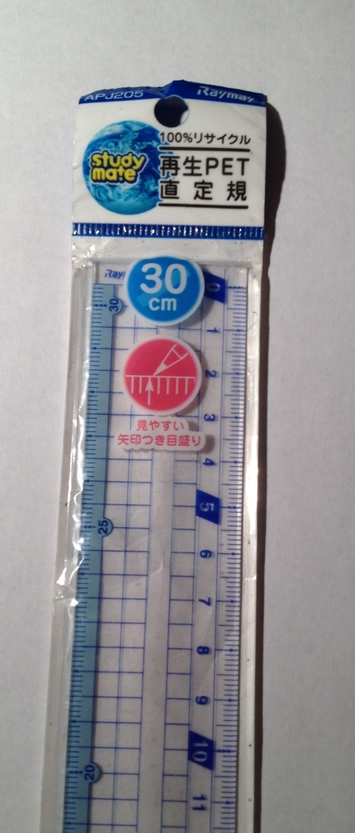
\includegraphics[width=0.25\textwidth]{ruler.jpg}
  \end{center}

  In what follows ``ruler'' means ``ruler with perpendicular markings''.

  \ii Draw a \textbf{large} diagram.
  It should ideally take up the entire page.
  It is not unreasonable to buy oversized paper
  ($17" \times 11"$ inches for example)
  in order to increase the maximal size of your diagram.

  \ii Bring \textbf{colored pens} to taste
  (i.e.\ if you're the kind of person that likes multi-colored diagrams).
  I certainly fell into this category:
  my diagrams often had red, blue, or green for emphasis.

%  \ii Bring a protractor if the contest allows it and you want to use it.
%  (The last time I checked, the IMO and USAMO do not.)
%  Personally, I never bothered with one.
\end{itemize}
Note that the last time I checked,
protractors were not allowed on either USAMO or IMO.

\section{Triangle centers}
General rule of thumb: when it is possible,
you should try to construct a point by using a ruler
instead of using a compass.
This is faster, easier, and less error-prone.
The one exception is that you get one circle (and its center) ``for free'':
it is impossible to make a mistake with the first circle that you draw.

With that in mind, suppose you have a problem with a triangle $ABC$.
\begin{itemize}
  \ii Always draw the \vocab{circumcenter} $O$ and circumcircle $\Gamma$ of $ABC$
  \emph{before} drawing the triangle itself.\footnote{I
    was appalled when I found out that some students will
    draw the triangle first, and then clumsily try to construct
      perpendicular bisectors to the three sides.
  This is too hard to get right.}
  That way, you have the point $O$ for free,
  and you can just pick any three points $A$, $B$, $C$ on that circle.

  \ii Always draw the circumcircle, even if it is not mentioned in the problem.

  \ii To construct the \vocab{incenter} $I$:
  take the perpendicular from $O$ through $BC$
  (using your ruler) and use it to find the
  arc midpoint $X$ of $\widehat{BC}$.
  Then line $AX$ is the $\angle A$-bisector.
  You can then intersect line $AI$ with the circle
  centered at $X$ with radius $XB=XC$ (by ``Fact 5'').
  Alternatively, construct the $B$-bisector.

  \ii To construct the incircle: construct $I$ as above,
  then take the foot $D$ of the perpendicular from $I$ to $\ol{BC}$,
  and draw the circle centered at $I$ through $D$.
\end{itemize}

In this way, we see that we can actually construct the incircle of a triangle
without having to do \emph{any} tricky compass constructions.
The only times we use the compass are at the very beginning
(to draw the circumcircle; it's impossible to get this wrong!)
and then to actually draw the incircle itself.

\begin{center}
\begin{asy}
size(7cm);
pair A = dir(110);
pair B = dir(210);
pair C = dir(330);

pair X = dir(270);
pair Y = dir(40);
filldraw(unitcircle, opacity(0.1)+lightblue, lightblue);
filldraw(A--B--C--cycle, opacity(0.1)+lightcyan, blue);

pair O = origin;
draw(O--X, heavygreen);
draw(O--Y, heavygreen);
draw(A--X, heavycyan);
draw(B--Y, heavycyan);

pair I = extension(A, X, B, Y);

dot("$A$", A, dir(A));
dot("$B$", B, dir(B));
dot("$C$", C, dir(C));
dot("$X$", X, dir(X));
dot("$Y$", Y, dir(Y));
dot("$O$", O, dir(315));
dot("$I$", I, dir(I));

/* TSQ Source:

A = dir 110
B = dir 210
C = dir 330

X = dir 270
Y = dir 40
unitcircle 0.1 lightblue / lightblue
A--B--C--cycle 0.1 lightcyan / blue

O = origin R315
O--X heavygreen
O--Y heavygreen
A--X heavycyan
B--Y heavycyan

I = extension A X B Y

*/
\end{asy}
\end{center}

Similarly,
\begin{itemize}
  \ii Constructing the \vocab{orthocenter} should be trivial,
  since you can draw the altitudes quickly with ruler alone.
  \ii Construct the \vocab{centroid} should be easy,
  since you have the midpoints of the sides
  (by simply taking the feet from $O$),
  so you can construct the medians with ruler alone.
\end{itemize}

Consequently, we see that
\begin{mdframed}
  \color{red}\bfseries
  It is possible to construct all four triangle centers
  using a compass only once, and at the very beginning.
\end{mdframed}
We also only need to use ``straightedge'' and ``perpendicular'' constructions,
i.e.\ we also avoid measuring angles with a protractor
or side lengths with a ruler.
Similarly, we don't have to build perpendicular bisectors or angle bisectors;
the relevant points are built in for us.
You can always do these more cumbersome operations if you like, of course,
and there are situations in which you will need to.
But it's nice to know that often you can avoid them.


\section{Drawing out of order}
\label{sec:phantom}
Since geometry is about some nontrivial coincidences
(three lines are concurrent, etc)
you can often draw the problem in a different order
in such a way that the diagram becomes easier to draw.

For example, consider the following problem.
\begin{example}
[USAMO 2009/1]
Given circles $\omega_1$ and $\omega_2$ intersecting at points $X$ and $Y$,
let $\ell_1$ be a line through the center of $\omega_1$
intersecting $\omega_2$ at points $P$ and $Q$
and let $\ell_2$ be a line through the center of $\omega_2$
intersecting $\omega_1$ at points $R$ and $S$.
Prove that if $P$, $Q$, $R$, and $S$ lie on a circle
then the center of this circle lies on line $XY$.
\end{example}
If you try to draw the points in the order listed, you are sunk:
the chance that $P$, $Q$, $R$, $S$ are cyclic
if you let $\ell_1$ and $\ell_2$ be arbitrary is basically zero.

Instead, let's draw $\omega_1$ and $\omega_2$
(with centers $O_1$ and $O_2$),
so that we have points $X$ and $Y$.
Then, instead of trying to draw $PQRS$, let's begin with the center $O$:
which we know should lie on line $XY$,
so we take an arbitrary such point on the line.

\begin{center}
\begin{asy}
size(6cm);
pair O_1 = dir(220);
pair O_2 = dir(320);
pair O = dir(110);
pair T = foot(O, O_1, O_2);
pair X = midpoint(O--T);
pair Y = 2*T-X;

filldraw(CP(O_1, X), opacity(0.1)+lightcyan, lightblue);
filldraw(CP(O_2, X), opacity(0.1)+lightcyan, lightblue);

draw(O--Y, red+dashed);

dot("$O_1$", O_1, dir(O_1));
dot("$O_2$", O_2, dir(O_2));
dot("$O$", O, dir(O));
dot("$X$", X, dir(100));
dot("$Y$", Y, dir(Y));

/* TSQ Source:

O_1 = dir 220
O_2 = dir 320
O = dir 110
T := foot O O_1 O_2
X = midpoint O--T R100
Y = 2*T-X

CP O_1 X 0.1 lightcyan / lightblue
CP O_2 X 0.1 lightcyan / lightblue

O--Y red dashed

*/
\end{asy}
\end{center}

Now, how do we locate $P$ and $Q$?
Well, we want that
\begin{itemize}
  \ii $OP = OQ$,
  \ii $O_2P = O_2Q$, and
  \ii $O_1$, $P$, $Q$ collinear.
\end{itemize}
The first two conditions imply $\ol{PQ} \perp \ol{OO_2}$:
so all we have to do is take the line through $O_1$
perpendicular to $\ol{OO_2}$, and intersect it with $\omega_2$.

\begin{center}
\begin{asy}
pair O_1 = dir(220);
pair O_2 = dir(320);
pair O = dir(110);
pair T = foot(O, O_1, O_2);
pair X = midpoint(O--T);
pair Y = 2*T-X;

filldraw(CP(O_1, X), opacity(0.1)+lightcyan, lightblue);
filldraw(CP(O_2, X), opacity(0.1)+lightcyan, lightblue);

draw(O--Y, red+dashed);

pair K = foot(O_1, O, O_2);
pair P = IP(O_1--K, CP(O_2, X));
pair Q = 2*K-P;
draw(O_1--Q, red);
draw(O--O_2, heavycyan);

dot("$O_1$", O_1, dir(O_1));
dot("$O_2$", O_2, dir(O_2));
dot("$O$", O, dir(O));
dot("$X$", X, dir(100));
dot("$Y$", Y, dir(Y));
dot("$P$", P, dir(120));
dot("$Q$", Q, dir(Q));

/* TSQ Source:

O_1 = dir 220
O_2 = dir 320
O = dir 110
T := foot O O_1 O_2
X = midpoint O--T R100
Y = 2*T-X

CP O_1 X 0.1 lightcyan / lightblue
CP O_2 X 0.1 lightcyan / lightblue

O--Y red dashed

K := foot O_1 O O_2
P = IP O_1--K CP O_2 X R120
Q = 2*K-P
O_1--Q red
O--O_2 heavycyan

*/

\end{asy}
\end{center}

Repeat for $R$ and $S$ and we have a diagram!

\begin{center}
\begin{asy}
pair O_1 = dir(220);
pair O_2 = dir(320);
pair O = dir(110);
pair T = foot(O, O_1, O_2);
pair X = midpoint(O--T);
pair Y = 2*T-X;

filldraw(CP(O_1, X), opacity(0.1)+lightcyan, lightblue);
filldraw(CP(O_2, X), opacity(0.1)+lightcyan, lightblue);

draw(O--Y, red+dashed);

pair K = foot(O_1, O, O_2);
pair P = IP(O_1--K, CP(O_2, X));
pair Q = 2*K-P;
draw(O_1--Q, red);
draw(O--O_2, heavycyan);

pair L = foot(O_2, O, O_1);
pair R = IP(O_2--L, CP(O_1, X));
pair S = 2*L-R;
draw(O_2--S, red);
draw(O--O_1, heavycyan);

draw(arc(O, abs(P-O), 180, 360), heavygreen);

dot("$O_1$", O_1, dir(O_1));
dot("$O_2$", O_2, dir(O_2));
dot("$O$", O, dir(O));
dot("$X$", X, dir(100));
dot("$Y$", Y, dir(Y));
dot("$P$", P, dir(120));
dot("$Q$", Q, dir(Q));
dot("$R$", R, dir(40));
dot("$S$", S, dir(S));

/* TSQ Source:

O_1 = dir 220
O_2 = dir 320
O = dir 110
T := foot O O_1 O_2
X = midpoint O--T R100
Y = 2*T-X

CP O_1 X 0.1 lightcyan / lightblue
CP O_2 X 0.1 lightcyan / lightblue

O--Y red dashed

K := foot O_1 O O_2
P = IP O_1--K CP O_2 X R120
Q = 2*K-P
O_1--Q red
O--O_2 heavycyan

L := foot O_2 O O_1
R = IP O_2--L CP O_1 X R40
S = 2*L-R
O_2--S red
O--O_1 heavycyan

!draw(arc(O, abs(P-O), 180, 360), heavygreen);

*/
\end{asy}
\end{center}

Now what you might notice in the diagram is that $\ol{PQ}$, $\ol{RS}$
and $\ol{XY}$ appear to be concurrent.
The reason for this is just radical axis:
the lines concur at the radical center of the three circles.
In fact, this gives us another way we could have constructed the diagram:
we could have just selected a point $Z$ on $\ol{XY}$,
and then taken lines $\ell_1$ and $\ell_2$ to pass through $Z$,
whence
\[ ZP \cdot ZQ = ZX \cdot ZY = ZR \cdot ZS. \]
then implies that $PQRS$ is cyclic.

If you understood all that, then in fact you are not really
very far from solving the problem.
And that highlights a small irony in the diagram-drawing process:
the closer you are to solving the problem,
the easier the diagram becomes to draw;
and yet the diagram is the thing that helps you solve the problem!

\section{Mechanical suggestions}
\subsection{Draw your first diagram the same way each time}
On any triangle $ABC$ problem, the first triangle I draw
always has basically the same proportions by default:
$\angle A \approx 60\dg$, $\angle B \approx 70\dg$, $\angle C \approx 50\dg$.
The diagram I gave in the previous section uses these proportions.

The nice thing about this is that
\alert{if you always use the same triangle
you can start to remember where things are} --- if a problem
turns out to involve a point that you've seen before,
then that point will be in \emph{the same physical location}.
(Sometimes this won't work out ---
certain points may be too far away to draw in your favorite triangle,
for example --- but you can still try.)

%This way, if you've done ten orthocenter problems
%and in the eleventh problem it turns out that
%a circle passes through the orthocenter,
%you're significantly more likely to notice this
%because the orthocenter has been in the same place each time.

As an example, consider the following four pictures.
\begin{center}
  \begin{minipage}[t]{6.5cm}
  \asyinclude{brazils/brazil-2011-p5.asy}
  \\ \centering \sffamily Brazil 2011/5
  \end{minipage}
  \quad
  \begin{minipage}[t]{6.5cm}
  \asyinclude{brazils/tstst-2016-p2.asy}
  \\ \centering \sffamily TSTST 2016/2
  \end{minipage}
  \\
  \begin{minipage}[t]{6.5cm}
  \asyinclude{brazils/tstst-2017-p1.asy}
  \\ \centering \sffamily TSTST 2017/1
  \end{minipage}
  \quad
  \begin{minipage}[t]{6.5cm}
  \asyinclude{brazils/sl-2005-g5.asy}
  \\ \centering \sffamily Shortlist 2005 G5
  \end{minipage}
\end{center}
Notice how you can see a certain point appearing in all four pictures,
despite the different name it comes with each time,
and the fact that it is defined differently in each problem.

\subsection{But check conjectures in different second diagrams}
That being said, if you have a conjecture, it's often worth the effort to
draw a second\footnote{or third, fourth, \dots} diagram and
\alert{see if it still looks true in different diagrams
before trying to spend a lot of time proving it}.

\subsection{Avoid circular reasoning with diagrams}
I personally find it helpful to not mark information on a diagram
if I don't know it's already true.\footnote{Some
  people go as far as to offset the diagram a little bit to
  avoid assumptions like this.
  I personally dislike this, but only weakly.}
What I mean by this:
\begin{itemize}
  \ii For example, if a problem asks me to show
  that $X$, $Y$, $Z$ are collinear,
  I will not draw the solid line $XY$,
  but rather will draw a dashed line to remind myself
  that this is the desired conclusion.
  \ii Similarly, if a problem asks me to show that four points
  $W$, $X$, $Y$, $Z$ are concyclic,
  I often will circle the four points, rather than drawing in the circle.
\end{itemize}
Often, using phantom points or otherwise
(like described in Section~\ref{sec:phantom}),
it's helpful to rephrase the problem in a way that makes
the ``missing'' information easier to draw.
For example, consider the following IMO problem.
\begin{example}
[IMO 2010]
Let $I$ be the incenter of a triangle $ABC$ and let $\Gamma$ be its circumcircle.
Let line $AI$ intersect $\Gamma$ again at $D$.
Let $E$ be a point on arc $\widehat{BDC}$ and $F$ a point on side $BC$ such that
\[ \angle BAF = \angle CAE < \tfrac12 \angle BAC. \]
Finally, let $G$ be the midpoint of $\overline{IF}$.
Prove that $\overline{DG}$ and $\overline{EI}$ intersect on $\Gamma$.
\end{example}
To draw this, I would rather draw in $K$ as the second intersection
of $\ol{EI}$ with $\Gamma$, then let $G = \ol{IF} \cap \ol{KD}$,
and then \emph{try to show $G$ is the midpoint},
since this is the piece of information which is the least
natural to mark in the diagram.
Thus one can draw a figure with all solid lines as below:
\begin{center}
\begin{asy}
size(8cm);

pair A = dir(110);
pair B = dir(210);
pair C = dir(330);
pair D = dir(-90);
pair I = incenter(A, B, C);
pair I_A = 2*D-I;

pair E = dir(295);
pair K = -E+2*foot(origin, E, I);
pair H = B*C/E;
pair F = extension(B, C, A, H);
pair G = extension(D, K, I, F);
pair P = extension(A, F, D, G);
pair Q = extension(I, P, I_A, F);

draw(A--B--C--cycle, lightblue);
filldraw(unitcircle, opacity(0.1)+lightcyan, lightblue);

draw(A--D, lightblue);
draw(F--A--E, heavygreen);
draw(E--K--D, orange);
draw(I--F, blue);
pair T = extension(B, C, A, D);

dot("$A$", A, dir(A));
dot("$B$", B, dir(B));
dot("$C$", C, dir(C));
dot("$D$", D, dir(220));
dot("$I$", I, dir(10));
// dot("$I_A$", I_A, dir(I_A));
dot("$E$", E, dir(E));
dot("$K$", K, dir(K));
// dot("$H$", H, dir(H));
dot("$F$", F, dir(F));
dot("$G$", G, dir(350));
// dot("$P$", P, dir(45));
// dot("$Q$", Q, dir(Q));
// dot("$T$", T, dir(T));
\end{asy}
\\
\sffamily Show that $G$ is the midpoint of $\ol{IF}$.
\end{center}
This makes it easier keep track of which
things I've proven and which things remain to show,
because the diagram now partially captures this information as well.
(This turns out to be the more natural way to think about
the problem, in any case.)


\section{How to mass-produce diagrams (controversial)}
\begin{quote}
  \sffamily
  ``Diagrams should not be drawn like Protoss but massed like Zerg\dots
  AZ once had a piece of paper covered with more than 20 bite-sized diagrams,
  and I gave him a high five when I saw this''
  --- James Tao
\end{quote}

I've given you advice on how to draw very nice diagrams with
ruler and compass, but you can also trade quality for quantity.

So here is a possible workflow that I haven't tried:
\begin{itemize}
  \ii Start by free-handing a very rough diagram,
  so you have a general sense of where the points in the picture lie.
  \ii Afterwards, draw (with ruler/compass) a single large nice diagram.
  \ii If you have a conjecture for something which is true,
  mass-produce a bunch of rough diagrams in order to see
  whether the conjecture looks true in all of them.
  \ii If you are stuck, mass-produce rough diagrams
  to try and find new conjectures.
  \ii Any time you have progress on the problem and want to think
  about it in a different way (for example using the intouch triangle $DEF$
  as the ``main'' triangle instead),
  draw a new nice diagram to reflect your updated intuition.
  \ii Any time you feel like drawing a new diagram, do so.
\end{itemize}

\section{Computer-Generated Figures}
Obviously this won't help much during the USAMO,
but for practice it is fun and besides the results are beautiful.

The two systems I use for digital figures are Geogebra and Asymptote.
I use Geogebra for its interactivity (when I am solving problems)
and Asymptote for its aesthetics (when I need to include a diagram as a PDF).
The workflow for both systems is quite similar.

\subsection{GeoGebra}
My main suggestion for Geogebra is:
\begin{mdframed}
  \bfseries\color{red}
  Use the GeoGebra command line for constructions whenever possible.
\end{mdframed}
This way you don't clutter your picture with unnecessary lines or circles.

Some technical suggestions for GeoGebra:
\begin{itemize}
  \ii GeoGebra lets you name objects from the command line:
  for example one can type \texttt{M = Midpoint[A,B]}.

  \ii GeoGebra 5+ has a command called \texttt{TriangleCenter[A,B,C,n]},
  so if you know the Kimberling center of a triangle quickly.
  The four most important ones are:
  \begin{itemize}
    \ii $I$ is the first Kimberling center
    \ii $G$ is the second Kimberling center
    \ii $O$ is the third Kimberling center
    \ii $H$ is the fourth Kimberling center
  \end{itemize}

  \ii Geogebra lets you define ``tools'' to make your life easier.

  You should define a tool called \texttt{Foot[X,A,B]} which builds
  the foot of the altitude form $X$ to $\ol{AB}$.
  Without this, you would instead have to type
  \texttt{Intersect[Line[A,B], PerpendicularLine[X,Line[A,B]]]}.

  See \url{https://www.geogebra.org/manual/en/Custom_Tools}
  for instructions on building tools.
  You can of course build more tools to taste.

  \ii To draw a segment, \texttt{Segment[A,B]} over \texttt{Line[A,B]}
  since it keeps your diagram cleaner.

  \ii GeoGebra supports vector addition: \texttt{2*M-A}
  gives you the reflection of $A$ over $M$.

  \ii Suppose $A \in \omega$, and $P$ is a point, and you want to construct
  the second intersection $B$ of line $AP$ with the circle.
  Then use \texttt{-A+2*Foot[O,P,A]} will do the trick,
  $O$ being the center of $\omega$.
  This may be worth making into a tool, but I haven't done so.

  \ii I prefer to keep grid-lines on but the axes off.

  \ii I prefer to only label points, and not label circles, segments, etc.
\end{itemize}

Let's give an example for all this.

\begin{example}
[HMMT 2016]
Let $ABC$ be a triangle with incenter $I$
whose incircle is tangent to $\overline{BC}$, $\overline{CA}$, $\overline{AB}$
at $D$, $E$, $F$.
Point $P$ lies on $\overline{EF}$ such that $\overline{DP} \perp \overline{EF}$.
Ray $BP$ meets $\overline{AC}$ at $Y$ and ray $CP$ meets $\overline{AB}$ at $Z$.
Point $Q$ is selected on the circumcircle of $\triangle AYZ$
so that $\overline{AQ} \perp \overline{BC}$.
Prove that $P$, $I$, $Q$ are collinear.
\end{example}

Here is how I construct it in GeoGebra
(again after having defined \texttt{Foot} as a tool, described above).
You start by selecting three points with the mouse;
then afterwards you only need the keyboard.
GeoGebra will autocomplete command names for you,
so this is fast.
\lstinputlisting{demos/hmmt-ggb.txt}

The resulting diagram looks as follows.
\begin{center}
  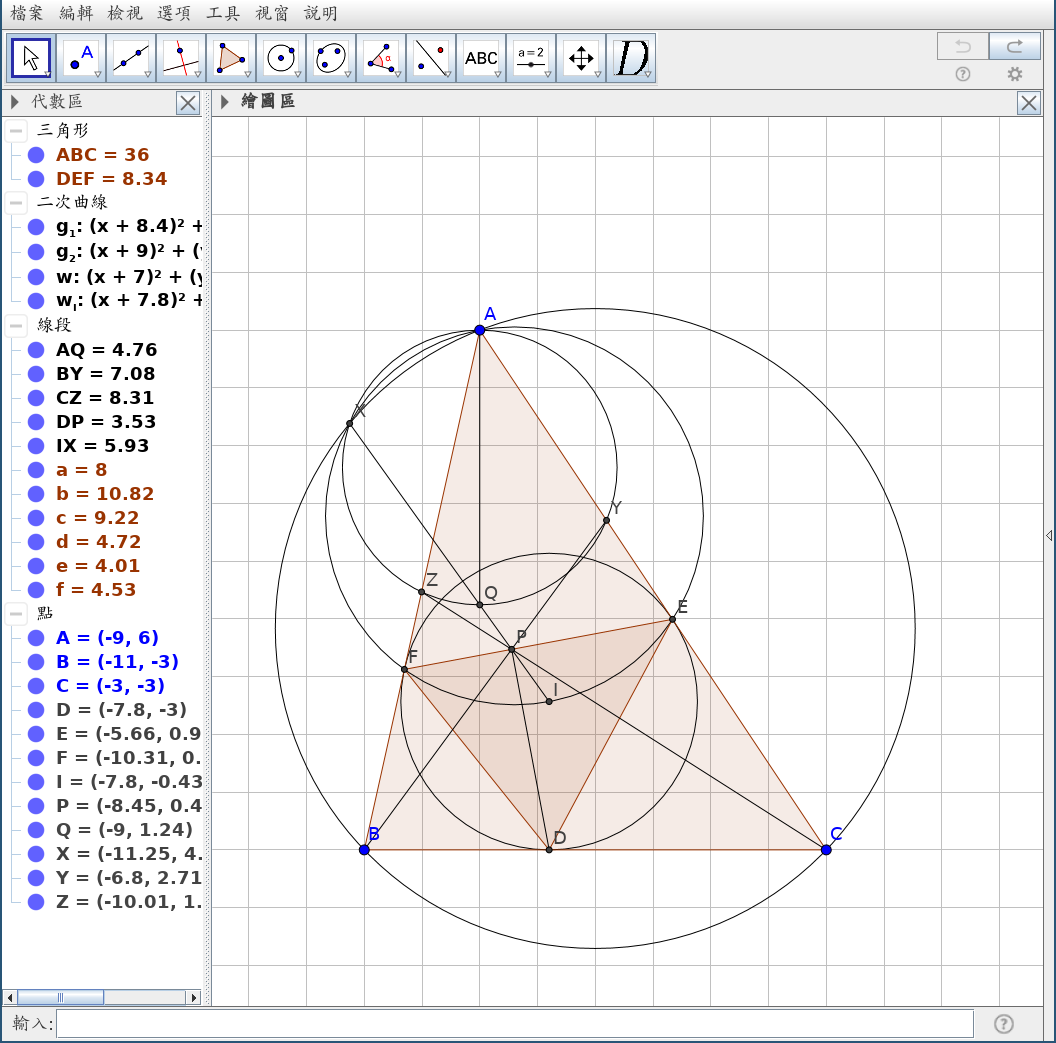
\includegraphics[width=0.99\textwidth]{demos/hmmt-demo.png}
\end{center}
This is pretty clean: none of the lines I don't want are in the picture.
The polygon is highlighted (\texttt{Polygon[\dots]} command) in red,
with the segments drawn in.
You can right click segments, circles, etc and adjust their colors as well,
or make some of them dashed, etc.
You can hide or show objects by clicking on the left panel.

Most importantly: you can drag the points $A$, $B$, $C$ around,
so \textbf{if you have a conjecture you want to verify,
just drag one of the points around a bit and see if it looks true}.
This is the number one reason why solving problems with Geogebra
diagrams is so much faster than on paper.

\subsection{Asymptote}
This is actually very similar to working with GeoGebra,
except the command names are different,
and you have to manually specify when to label/draw a point.

Asymptote is notoriously tricky to install alongside \LaTeX,
unless you are on Linux\footnote{\texttt{sudo pacman -S asymptote} on Arch,
\texttt{sudo apt-get install asymptote} on Ubuntu/Debian, \dots}.
But doing this set-up right is worth it,
because it will make diagrams much easier.
You can read the Asymptote guide at
\url{https://web.evanchen.cc/asyguide.html}
for some hints on how to set this up.

Anyways, maybe it is better if I just give an example.
Here is the same diagram, redrawn by me in Asymptote.
\begin{center}
  \asyinclude{demos/hmmt.asy}
\end{center}
Here is the code that generated it.
\lstinputlisting[language=C]{demos/hmmt.asy}

If you look through source codes for my geometry handouts,
you can find many more such Asymptote examples.

(Also worth mentioning: GeoGebra can actually export to Asymptote.)

\end{document}
